\documentclass[tikz,border=10pt]{standalone}
\usepackage[utf8]{inputenc}
\usepackage{tikz}
\usetikzlibrary{shapes, arrows.meta, positioning, calc, shadows.blur, backgrounds, fit}

% Paleta de colores consistente
\definecolor{paperPurple}{RGB}{147, 112, 219} % MediumPurple para Sequence/Transformer
\definecolor{paperOrange}{RGB}{255, 165, 0}  % Orange para Demographics (Tabular)
\definecolor{paperGray}{RGB}{119, 136, 153}  % LightSlateGray para Fusion
\definecolor{paperBlue}{RGB}{70, 130, 180}   % SteelBlue para Embeddings básicos

\begin{document}

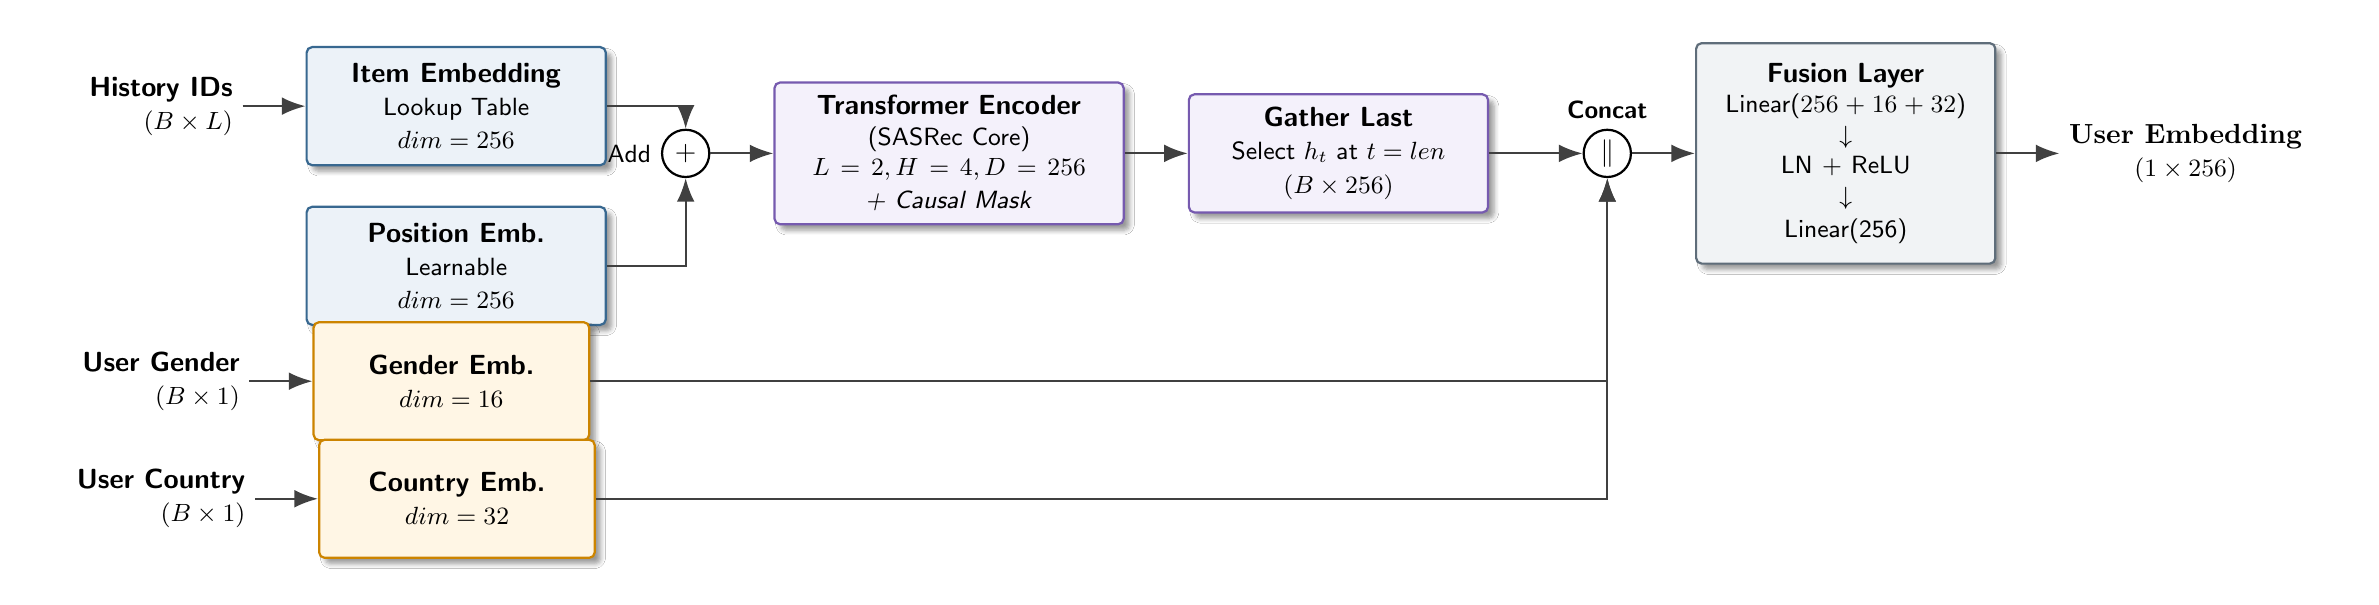
\begin{tikzpicture}[
    node distance=1.0cm and 1.2cm,
    font=\sffamily\normalsize,
    % Estilo base para bloques
    block/.style={
        draw, 
        rounded corners=2pt, 
        minimum height=1.5cm, 
        minimum width=3.8cm, 
        align=center,
        blur shadow={shadow blur steps=5},
        thick
    },
    % Estilo para inputs
    input_node/.style={
        align=right,
        font=\sffamily\bfseries\normalsize
    },
    % Estilo para flechas
    arrow/.style={
        -{Latex[length=3mm]}, 
        thick, 
        darkgray
    },
    % Operadores (Suma y Concat)
    operator/.style={
        circle, 
        draw, 
        thick, 
        fill=white, 
        inner sep=1pt, 
        minimum size=0.6cm
    }
]

    % --- 1. Rama Principal: Secuencia de Interacciones (SASRec) ---
    
    % Input Sequence
    \node[input_node] (in_seq) {
        History IDs\\
        \small $(B \times L)$
    };

    % Item Embedding
    \node[block, draw=paperBlue!80!black, fill=paperBlue!10, right=0.8cm of in_seq] (item_emb) {
        \textbf{Item Embedding}\\
        \small Lookup Table\\
        \small $dim=256$
    };
    \draw[arrow] (in_seq) -- (item_emb);

    % Position Embedding (Se suma, no es input externo)
    \node[block, draw=paperBlue!80!black, fill=paperBlue!10, below=0.5cm of item_emb] (pos_emb) {
        \textbf{Position Emb.}\\
        \small Learnable\\
        \small $dim=256$
    };

    % Suma (Add)
    \node[operator, label={180:\small Add}] (add_op) at ($(item_emb.east) + (1.0, -0.6)$) {$+$};


    % \node[circle, draw, thick, fill=white, inner sep=1pt, minimum size=0.6cm, label={180:\sffamily\bfseries\small Concat}] (concat) at (concat_point) {$\parallel$};
    
    % Conexiones a la suma
    \draw[arrow] (item_emb.east) -| (add_op);
    \draw[arrow] (pos_emb.east) -| (add_op);

    % Transformer Block (SASRec Core)
    \node[block, draw=paperPurple!80!black, fill=paperPurple!10, right=0.8cm of add_op, text width=4.2cm, minimum height=1.8cm] (transformer) {
        \textbf{Transformer Encoder}\\
        \small (SASRec Core)\\
        \small $L=2, H=4, D=256$\\
        \textit{\small + Causal Mask}
    };
    \draw[arrow] (add_op) -- (transformer);

    % Gather Last State (Extract h_L)
    \node[block, draw=paperPurple!80!black, fill=paperPurple!10, right=0.8cm of transformer] (gather) {
        \textbf{Gather Last}\\
        \small Select $h_t$ at $t=len$\\
        \small $(B \times 256)$
    };
    \draw[arrow] (transformer) -- (gather);


    % --- 2. Rama Demográfica (Inferior) ---
    
    % Inputs
    \node[input_node, below=2.5cm of in_seq] (in_gender) {User Gender\\ \small $(B \times 1)$};
    \node[input_node, below=0.5cm of in_gender] (in_country) {User Country\\ \small $(B \times 1)$};

    % Embeddings Demográficos
    \node[block, draw=paperOrange!80!black, fill=paperOrange!10, right=0.8cm of in_gender, minimum width=3.5cm] (gender_emb) {
        \textbf{Gender Emb.}\\
        \small $dim=16$
    };
    
    \node[block, draw=paperOrange!80!black, fill=paperOrange!10, right=0.8cm of in_country, minimum width=3.5cm] (country_emb) {
        \textbf{Country Emb.}\\
        \small $dim=32$
    };

    \draw[arrow] (in_gender) -- (gender_emb);
    \draw[arrow] (in_country) -- (country_emb);

    % --- 3. Concatenación y Fusión ---

    % Punto de concatenación
    % Alineado horizontalmente con 'gather' y verticalmente centrado entre las ramas
    \coordinate (concat_x) at ($(gather.east) + (1.5, 0)$);
    \coordinate (concat_y) at ($(gather.east)!0.5!(gender_emb.east)$); % Punto medio Y
    
    % Nodo Concat
    \node[operator, label={90:\sffamily\bfseries\small Concat}] (concat) at (concat_x |- gather) {$\parallel$};

    % Rutas hacia Concat
    \draw[arrow] (gather) -- (concat);
    
    % Rutas complejas para demográficos
    \draw[arrow] (gender_emb.east) -| (concat);
    \draw[arrow] (country_emb.east) -| ($(concat) + (0, -0.8)$) -- (concat);

    % Fusion Layer Final
    \node[block, draw=paperGray!80!black, fill=paperGray!10, right=0.8cm of concat, minimum height=2.8cm, text width=3.5cm] (fusion) {
        \textbf{Fusion Layer}\\
        \small Linear($256+16+32$)\\
        $\downarrow$\\
        \small LN + ReLU\\
        $\downarrow$\\
        \small Linear(256)
    };
    \draw[arrow] (concat) -- (fusion);

    % Output Final
    \node[right=0.8cm of fusion, font=\bfseries, align=center] (out_final) {
        User Embedding\\
        \small $(1 \times 256)$
    };
    \draw[arrow] (fusion) -- (out_final);


    % --- Fondo (Opcional) ---
    \begin{scope}[on background layer]
        \node[fit=(in_seq)(in_country)(out_final), fill=white, inner sep=0.5cm] {};
    \end{scope}

\end{tikzpicture}
\end{document}